The allocate algorithm generalizes the compact algorithm described in \autoref{sec-compact}.
Before reading this section it is advised to read \autoref{sec-compact}.
The compact algorithm generates a single output for each input that is evaluated as \textit{true}, according to a given predicate, and generates no output elements for input values which are evaluated to \textit{false}.
The allocate algorithm can compute a number of output elements dynamically for each input element.
The main difference is that the transformation function of $f_{P}(S)_{new}$ does not translate to only zeros and ones, but into \textit{n} needed allocation requests.
The idea is illustrated in \autoref{fig:allocate} and as can be seen the predicate function here ranges with values from zero to three as opposed only zero and one as in the compact algorithm.
\begin{figure}[ht]
	\centering
	\fbox{
		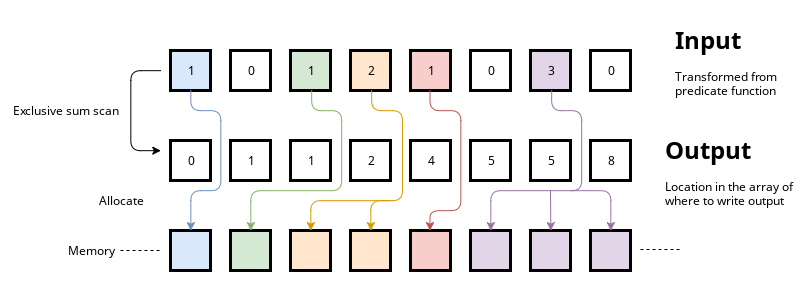
\includegraphics[width=0.85\textwidth]{figs/algorithm/allocate.png}
	}
	\caption{Example of allocate}
	\label{fig:allocate}
\end{figure}
The steps in the allocate algorithm are the same as described in \autoref{alg-compact}.
Usage of this kind of algorithm is very use case specific, but in general if it is desired to do a compact operation on varying sizes of objects then this algorithm makes it possible to achieve this.

%TODO: maybe small code example but ommit if no time